% In this section you should describe what you have done in sufficient detail to enable another research or team to repeat your study. Depending on your project, you will need to include a description of and justification for the experimental design, code development, details of data analysis, and production of results. Some details of the methods could be included in an Appendix.

\chapter{Methodology}

\section{Dataset}
This project utilizes the MIMIC-IV dataset \cite{mimiciv} which is a publicly available, de-identified database of patient records from the Beth Israel Deaconess Medical Center, covering ICU admissions between 2008 and 2019. We utilized the discharge summaries made available through this dataset which provide functional status information of patients in free-text notes. \\

The subset used for analysis comprises approximately 3.28 GB of unstructured clinical text. These summaries were chosen for their richness and relevance to both unsupervised and supervised learning tasks.\\

Access to the data was obtained via the PhysioNet credentialing process, which involves completing data usage training and agreeing to ethical use guidelines. 


\section{Pre-processing}
The text preprocessing pipeline includes the following steps:

\begin{itemize}
    \item \textbf{Sentence Segmentation:} Raw clinical texts (discharge summaries from the \texttt{discharge.csv} file in the MIMIC-IV dataset) are segmented into individual sentences using the spaCy NLP library, which applies rule-based syntactic parsing to identify sentence boundaries.

    \item \textbf{Text Preprocessing:} Sentences are cleaned by removing markdown syntax, list indicators, and excess whitespaces to reduce noise and standardize formatting.

    \item \textbf{Filtering:} Sentences that are too short, purely numeric, or lack alphabetic characters are excluded to retain only linguistically and semantically meaningful entries.
\end{itemize}

The cleaned sentences are compiled into a structured tabular format, suitable for downstream machine learning tasks and manual annotation workflows for both supervised and unsupervised models.

 
\section{Design of Unsupervised models}

\subsection{LDA with TF and K-Means with ClinicalBERT}

To retain semantic meaning in clustering discharge summary sentences, two approaches were used:

\begin{itemize}
    \item \textbf{Term Frequency with LDA:} LDA was applied to term frequency vectors to identify interpretable clinical topics based on word co-occurrence. This method captures the broader thematic structure in the text.
    
    \item \textbf{K-Means with ClinicalBERT:} ClinicalBERT embeddings provide context-aware representations tailored to medical language. Applying K-Means to these embeddings enables unsupervised grouping of semantically similar sentences, even when they differ in wording. ClinicalBERT was selected for its domain-specific training on clinical notes, thereby making clusters based on the semantic relevance of text-processed tokens.
\end{itemize}

Using both methodologies provides complementary perspectives, LDA captures latent topic structures through word co-occurrence patterns, while the ClinicalBERT with Kmeans clustering captures semantic similarity using contextual embeddings. This dual approach allows for a comparative analysis of clustering quality and interpretability. Both of these approaches were implemented with scalable python frameworks such as PySpark to enable the algorithms to run on High Performance Computing (HPC)\footnote{The relevant code for scalable clustering models can be found here: \url{https://github.com/twinzies/fsi-nlp} and also at \url{https://github.com/AlessandroPerelli/com6911-teamdn1/tree/main/unsupervised_model/fsi-nlp} This complements the code that can be run on limited computational resources such as a PC: \url{https://github.com/AlessandroPerelli/com6911-teamdn1/tree/main/unsupervised_model/kmeans-ClinicalBERT}} \medskip


In the LDA approach, bag-of-words and term frequency representations were used to generate topic distributions. For the K-Means approach, word-level embeddings were generated using ClinicalBERT. These embeddings enabled the clustering of semantically similar sentences. Both methods were compared with traditional feature extraction techniques to evaluate their effectiveness. The probabilistic formulation of LDA is given by the following generative process.

\begin{align*}
\theta_d &\sim \text{Dirichlet}(\alpha) \quad \text{(document-topic distribution)} \\
z_{dn} &\sim \text{Multinomial}(\theta_d) \quad \text{(topic assignment)} \\
w_{dn} &\sim \text{Multinomial}(\beta_{z_{dn}}) \quad \text{(term from topic)}
\end{align*}

The joint probability models the generative process of the documents, enabling the discovery of latent semantic structures based on term frequency inputs. This formulation is expected to allow the LDA approach to effectively uncover underlying topic patterns across the corpus. The joint probability is given by:
\[
P(\theta, z, w \mid \alpha, \beta) = \prod_{d=1}^{D} P(\theta_d \mid \alpha) \prod_{n=1}^{N_d} P(z_{dn} \mid \theta_d) P(w_{dn} \mid z_{dn}, \beta)
\]

Where,
$w_{dn}$ = term frequency (TF) of the $n$-th word in document $d$, 
$z_{dn}$ = topic assigned to word $w_{dn}$, 
$\theta_d$ = topic distribution for document $d$, 
$\beta$ = topic-word distribution, 
$\alpha$ = Dirichlet prior for $\theta$. \bigskip

In this formulation, $K$, the number of topics, determines the dimensionality of the document-topic distribution $\theta_d$, the set of possible topic assignments $z_{dn}$, and the size of the topic-word distribution matrix $\beta$. Though not explicitly shown in the equations, $K$ governs the latent structure over which the LDA model is defined.\bigskip

KMeans clustering, applied to ClinicalBERT embeddings, is formalized by the following objective function.

\[
\underset{C}{\arg\min} \sum_{i=1}^{k} \sum_{x \in C_i} \| x - \mu_i \|^2
\]

Where, 
$x$ = ClinicalBERT embedding of the tokens of the document, 
$k$ = number of clusters, 
$C_i$ = set of points assigned to cluster $i$, 
$\mu_i$ = centroid of cluster $i$, computed as:
\[
\mu_i = \frac{1}{|C_i|} \sum_{x_j \in C_i} x_j
\]


\subsection{Rule Based with K-Means}

\begin{itemize}
    \item Rule-based labelling: Part A of Hybrid model consisting of preprocessing, which includes lowercasing, punctuation removal, tokenization, and lemmatization using NLTK. Initially, sentences were matched against manually crafted keywords and phrase dictionaries consisting of 4-ICF aligned categories. Each dictionary consists of around 30 keywords and domain-specific phrases. A sentence was given a Rule-based label if it matched at least one phrase or keyword. This resulted in high precision initial labelling, with keeping unlabeled sentences untouched. 
    \item BioBERT with k-means: Further in Part B of Hybrid model, Sentences embeddings were created using BioBERT model with a 768-dimensional output. K Means clustering was used with k=10, n\_init=10 over the group of around 50,000 sentences based on semantic similarity. For each cluster, label purity was measured based on the existing Rule-based labels. If the dominant label accounted for more than 80\% of the labelled sentences in that particular cluster, and the cluster size was more than n=30, the label was propagated to all the previously unlabeled sentences within that cluster that had a token count of at least 5, to remove any accidental labellings. \\
\end{itemize}
This two-staged hybrid approach enabled both high-confidence initial annotation through manually derived rules and broader semantic generalization through unsupervised clustering. While the approach was highly effective and did as expected in capturing structured FSI- related content– particularly in categories such as Mobility and Communication \& Cognition, which presented higher precision – manual inspection revealed challenges and difficulties faced by the model in categories like IPIR and SC/DL, where key-word based rules and embedding similarity often struggled with contextual ambiguity. Nevertheless, the combination of rule-based and clustering based components provided a flexible, interpretable framework for early-stage annotation of FSI statements in low-resource settings

 
\section{Design of Supervised models}

\subsection{Annotations}

In order to develop supervised models, we needed to manually annotate our data as mentioned before. To do this, we divided the data (around 44000 lines) between five team members. After labels were assigned with reference to the ICF annotation guidelines \cite{CommCognitionGuideline2023} \cite{MobilityGuideline2023} \cite{InterpersonalGuideline2023}, the team cross-validated the labeling and annotation efforts. Then the splits were combined to form various datasets for experimentation and model development:

\begin{itemize}
    \item Full dataset - contains every annotated sentence, including all 0 labels.
    \item Label dataset - contains every annotated sentence, excluding all 0 labels.
    \item Category-specific datasets - four separate files, one for each ICF category, each containing all sentences that carry that label (and only that label).
    \item Multi-label only dataset - this dataset contains all the sentences which have two or more labels.
\end{itemize}

\subsection{CNN-RNN}

One of the models implemented was a CNN-RNN hybrid model. This model uses pre-trained FastText embeddings, a convolutional layer with ReLU activation and adaptive max-pooling, a recurrent layer, specifically GRU, is used as it is more lightweight than LSTM, a dropout layer to mitigate overfitting, and a fully-connected output layer. Finally, this model makes its multi-label predictions using a sigmoid activation function that produces independent probabilities for each label with a decision threshold of 0.5 for each class assignment, allowing the model to assign multiple labels to a singular sentence. Binary cross-entropy loss is applied to all four labels, and an Adam optimiser is implemented. Early stopping is also used with a patience of 3 in order to stop over-fitting in the model. Though this is a reasonably lightweight model, the negative samples (sentences labelled 0) were undersampled by 95\% in order to create a more even split between the positive and negative sentences and cut down on training time. A stratified split was used to create train, test and validation sets to ensure an even split of all four labels. Fig.~\ref{fig:cnn-rnn-arch} shows a diagram of the model's architecture. \\

\begin{figure}
    \centering
    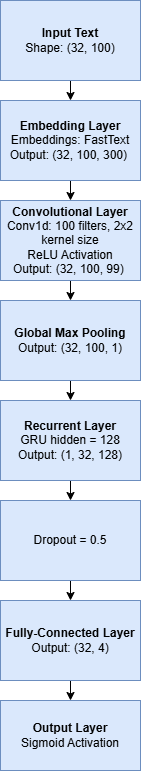
\includegraphics[width=0.1\linewidth]{myReport/figures/CNN-RNN.drawio.png}
    \caption{CNN-RNN Hybrid Model Architecture}
    \label{fig:cnn-rnn-arch}
\end{figure}

 
\subsection{FNN}
Another model we explored was an FNN. FNN's are commonly used for NLP tasks, so this model is not only suitable for this task, but provides for a good comparison with the CNN-RNN hybrid model. This FNN relies on a simple bag-of-embeddings representation of each sentence. All tokens are first projected into 300-dimensional pre-trained FastText vectors (the same used in the CNN-RNN hybrid model). Padding tokens are masked out and the remaining embeddings are mean-pooled to give a single, fixed-length sentence vector. \\

This vector is then passed through two fully connected hidden layers of 256 and 128 units, each followed by a ReLU activation and a 0.5 dropout layer to reduce over-fitting. A final linear layer with sigmoid activation produces four independent probabilities, one for each ICF category and a decision threshold of 0.5 converts these probabilities into binary labels, allowing multiple categories to be assigned simultaneously. Training follows the same procedure used for the CNN-RNN hybrid model for ease of comparison. This is:

\begin{itemize}
    \item Vocabulary is capped at 1000 tokens and sentences are truncated/padded to 100 tokens.
    \item The dominant “no-label” samples (category 0) are under-sampled by 95\% to balance the four positive classes and reduce training time.
    \item A 64/16/20 split is used for train, validation and test sets to preserve label distribution.
    \item Optimisation uses binary cross-entropy loss, the Adam optimiser ( with a learning rate of 0.001 and a batch size of 32) and early stopping with a patience of 3 based on validation micro-F1.
    \item Embedding weights (except the padding vector) are fine-tuned during training, keeping the model lightweight and computationally efficient.
\end{itemize}

\subsection{Random Forest}
The final model we implemented is a Random Forest classifier using a hybrid model that combines TF-IDF and FastText embeddings to classify clinical sentences into functional status categories. TF- IDF captured the most important words from the text while FastText provided a deeper meaning by focusing on each word and turning it into a dense vector using pre-trained vector embeddings. These two features were then combined to give the model both lexical and semantic information. The classifier was then set up to handle multi-labels classification which means that it could assign more than one label like Mobility, Self-care and Domestic life, Interpersonal Interactions and Relationships, Communication and Cognition to each of the sentences. We used 100 trees in the forest and set a maximum depth of 20 to balance accuracy and efficiency. Since the test data was not labeled, we evaluated the model on training data using precision, recall and F1-score and then visualized the results using a bar chart. We have also plotted how many times each label is  predicted in the test set and also printed 30 predicted sentences to see how our model performed. While the model worked well with Mobility related information, it struggled with less common categories due to the class imbalance and the lack of more advanced techniques like class weighting or sampling. Still, this method was fast, interpretable, and useful as a starting point for functional status classification\footnote{The relevant code for supervised models can be found here \url{https://github.com/AlessandroPerelli/com6911-teamdn1/tree/main/supervised_model}.}. \medskip


\section{Evaluation}

% Evaluated with micro-F1 because of the imbalanced classes. 
\subsection*{Unsupervised Models}

Due to the lack of reliable ground truth labels for most of the dataset, we evaluate unsupervised models using a combination of cluster performance metrics—such as silhouette scores and perplexity—and qualitative methods including visual inspection and topic exploration through word clouds. All unsupervised algorithms are developed using PySpark to ensure scalability and are executed on a high-performance computing (HPC) environment to efficiently process large volumes of text data.\medskip

\subsection{Scalable ClinicalBERT with K-Means Clustering}

We generate sentence embeddings using ClinicalBERT and apply K-Means clustering to group semantically similar content. We assess cluster quality using silhouette scores, which quantify how well each sentence fits within its assigned cluster relative to others. To support visual interpretation, we use dimensionality reduction techniques such as t-SNE and PCA, enabling 3D visualizations of the clustering structure. For interpretability, we construct word clouds based on the most frequent terms within each cluster to highlight the dominant themes.\medskip

\subsection{Scalable LDA with Term Frequency}

We implement Latent Dirichlet Allocation (LDA) on tokenized text data, following preprocessing steps including stemming, lemmatization, and stop word removal. Since LDA operates on term frequency rather than contextual embeddings, we use raw term counts as input. We evaluate model performance using perplexity scores, where lower values indicate better generalization. Additionally, we manually review the top words within each topic to assess semantic coherence and thematic relevance.

\subsection{Rule-Based with K-Means Approach}

Without ground truth labels, we evaluated our rule-based K-Means method using internal metrics and manual review. We assigned initial labels using handcrafted keyword dictionaries for four ICF categories, then generated BioBERT embeddings for sentence representations. Using K-Means ($k=10$), we clustered semantically similar sentences. We propagated labels within high-purity clusters (defined as those with more than 80\% of sentences sharing the same rule-based label and at least 30 samples). \\

For visualization, we reduced dimensions with UMAP to inspect cluster distribution against functional categories. Manual review confirmed strong performance for Mobility and Communication \& Cognition categories, with less consistency in ambiguous categories like Interpersonal Interactions \& Relationships and Self-care \& Domestic Life The hybrid approach effectively expanded our labeled dataset semi-automatically while maintaining interpretability and resource efficiency.


\subsection{Supervised Models}

We evaluated our supervised models using standard multi-label metrics: \textbf{precision}, \textbf{recall}, and \textbf{F1-score} (micro and macro averages). Accuracy is not a suitable metric for this problem due to the imbalanced classes in the dataset and therefore was not used for evaluation. Data was split 64\%/16\%/20\% (train/validation/test) with stratification to maintain label balance. A confusion matrix and learning curves for each of the neural models was also produced. \\

The \textbf{CNN-RNN} model performed best overall, especially for well-performing categories like \textit{Mobility} and \textit{Communication \& Cognition}. Our \textbf{FNN} model was lighter and faster while remaining competitive. Both neural models used validation micro-F1 for early stopping to prevent overfitting.\\

Our \textbf{Random Forest} model, which used combined TF-IDF and FastText features, performed adequately for frequent labels but struggled with class imbalance and lacked the expressiveness of deep models. Without a proper test set, Random Forest evaluation relied on training data and qualitative assessment.
